\subsection{Verifica del software}

\subsubsection{Versioni del browser supportate}
\begin{figure}[h]
	\centering
	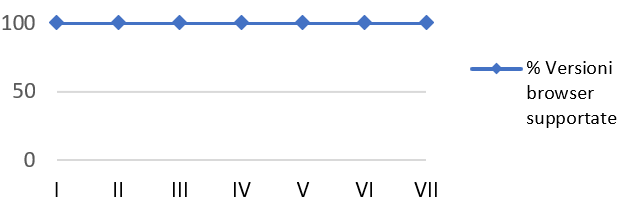
\includegraphics[width=11cm]{Images/vBrowser}
	\caption{Percentuale delle versioni browser supportate.}
\end{figure}

\subsubsection{Facilità di utilizzo}
\begin{figure}[h]
	\centering
	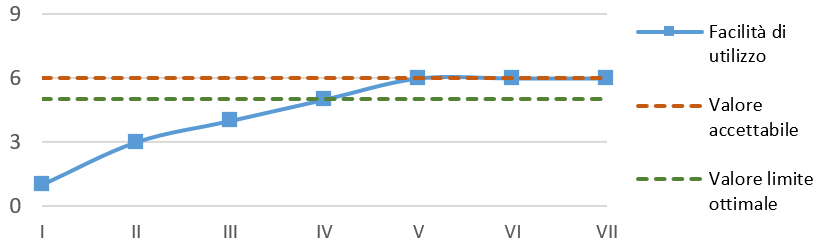
\includegraphics[width=13cm]{Images/facUtilizzo}
	\caption{Facilità di utilizzo in base al numero di click.}
\end{figure}

\subsubsection{Copertura dei requisiti}
\begin{figure}[h]
	\centering
	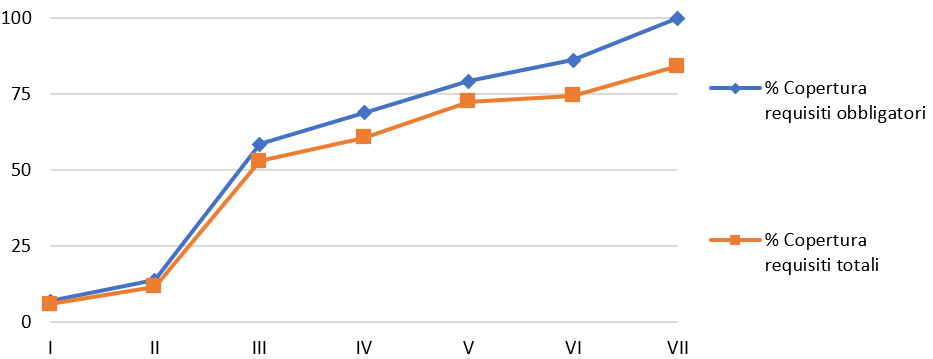
\includegraphics[width=14cm]{Images/copRequisiti}
	\caption{Percentuale dei requisiti soddisfatti.}
\end{figure}

\subsubsection{Average Cyclomatic complexity}
\begin{figure}[h]
	\centering
	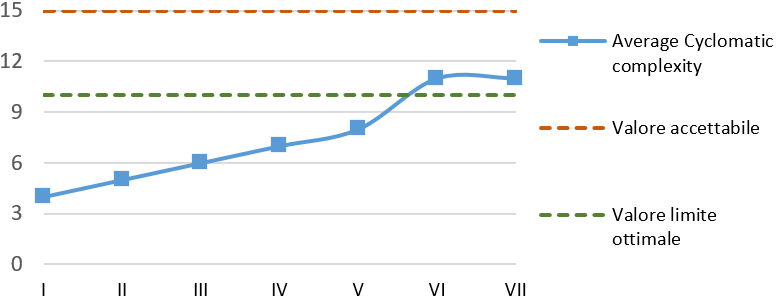
\includegraphics[width=14cm]{Images/avComplex}
	\caption{Andamento della complessità ciclomatica.}
\end{figure}

\subsubsection{Tempo medio di risposta}
\begin{figure}[h]
	\centering
	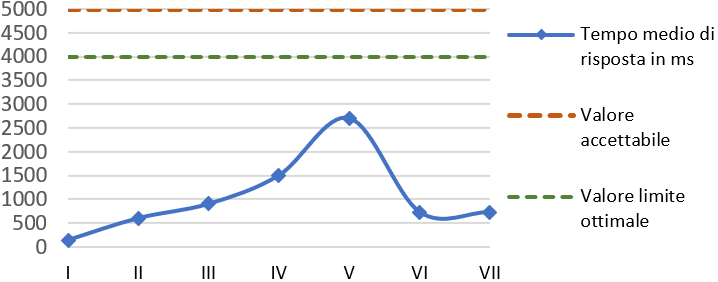
\includegraphics[width=14cm]{Images/tRisp}
	\caption{Andamento della risposta media.}
\end{figure}

\newpage

\subsubsection{Facilità apprendimento funzionalità}
\begin{figure}[h]
	\centering
	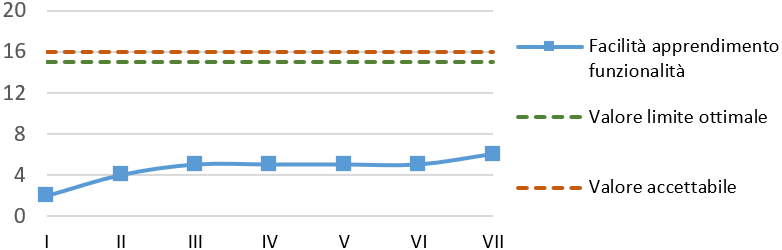
\includegraphics[width=16cm]{Images/fAppr}
	\caption{Facilità di apprendimento in base ai minuti utilizzati.}
\end{figure}